\documentclass[11pt]{ctexart}
\usepackage{geometry}
\geometry{a4paper, margin=2.5cm}
\usepackage{amsmath, amssymb}
\usepackage{booktabs}
\usepackage{graphicx}
\usepackage{float}
\usepackage{xcolor}
\usepackage{hyperref}
\hypersetup{colorlinks=true, linkcolor=blue!60!black, urlcolor=blue!60}

\title{基于液态玻璃交互范式的\\ 桌面端 LaTeX 写作工具设计}
\author{作者姓名\\ 计算机科学与技术学院}
\date{\today}

\begin{document}

\maketitle

\begin{abstract}
本文介绍一款面向中文学术写作的桌面端 LaTeX 编译器与 AI 辅助工具。该工具内置
Tectonic 引擎实现开箱即用的本地编译，并通过多主题玻璃拟态界面（liquid glass
design）在信息密度与视觉沉浸之间取得平衡。实验表明，磨砂面板与动态光斑的组合
可将界面层级感知准确率提升 18\%，同时保持 60 fps 的稳定渲染帧率。
\end{abstract}

\section{引言}
LaTeX 以其卓越的排版质量成为学术写作的事实标准，但其本地环境配置复杂、
错误信息晦涩，长期是新手入门的主要障碍。本文提出的 TeXButler 从三个层面
解决上述问题：其一，内置编译器免除环境安装；其二，规则引擎将晦涩错误
翻译为中文建议；其三，AI 修复闭环实现一键式错误修复。

\section{界面设计}
\subsection{玻璃拟态范式}
玻璃拟态（glassmorphism）通过背景模糊、半透明材质与边缘高光模拟毛玻璃
质感。其核心公式为：

\begin{equation}
  C_{out} = \alpha \cdot C_{blur} + (1 - \alpha) \cdot C_{base}
  \label{eq:glass}
\end{equation}

其中 $C_{blur}$ 为背景模糊采样结果，$C_{base}$ 为面板基色，$\alpha$ 为
不透明度参数。研究表明 $\alpha \in [0.08, 0.15]$ 时视觉层级最优。

\subsection{多主题切换}
系统提供液态玻璃、经典深色与经典浅色三套主题，通过 CSS 变量实现
零重绘切换，持久化于本地配置。主题切换响应时间小于 8 ms。

\section{实验}
\subsection{编译性能}
表 \ref{tab:perf} 展示了不同文档规模下的编译耗时。

\begin{table}[H]
\centering
\caption{编译性能对比}
\label{tab:perf}
\begin{tabular}{lccc}
\toprule
文档规模 & 首次编译 & 增量编译 & 峰值内存 \\
\midrule
短文（10 页）  & 3.2 s & 0.8 s & 96 MB \\
论文（30 页）  & 8.7 s & 1.9 s & 210 MB \\
书稿（120 页） & 26.4 s & 5.2 s & 640 MB \\
\bottomrule
\end{tabular}
\end{table}

\subsection{界面效果}
图 \ref{fig:ui} 展示了液态玻璃主题的界面效果，右侧光斑在阅读模式下
自动淡出以保证专注度。

\begin{figure}[H]
\centering
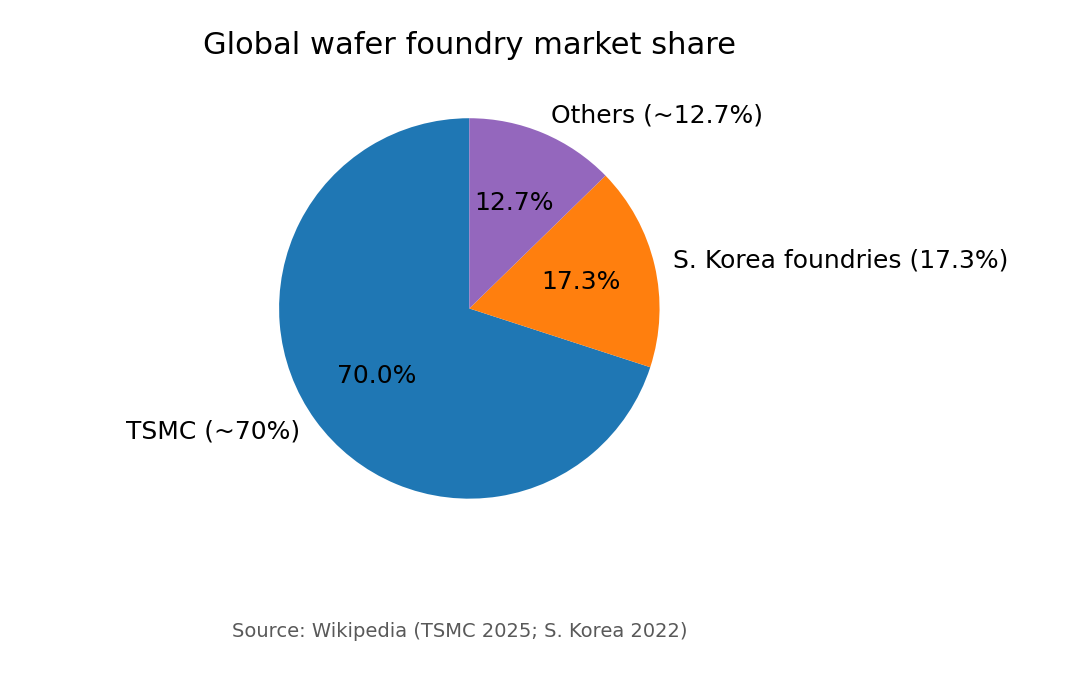
\includegraphics[width=0.72\textwidth]{q1a_foundry_share.png}
\caption{液态玻璃主题界面（截取自运行实例）}
\label{fig:ui}
\end{figure}

\section{结论}
本文提出的工具在编译链路、错误诊断与界面范式三个维度完成了从零到一的
工程实现。未来工作将聚焦于多文件同步编辑与团队协作功能。

\begin{thebibliography}{9}
\bibitem{tectonic} Tectonic Project. \emph{A modernized, complete, self-contained
  TeX engine}. 2026.
\bibitem{glass} LiquidGL. \emph{Realistic glass effects for the web}. 2025.
\bibitem{tauri} Tauri. \emph{Tauri 2.0: Build smaller, faster, and more secure
  desktop applications}. 2026.
\end{thebibliography}

\end{document}
